\section{Introduction}
\label{sec:intro}

%%
%% Circumstances when bowshocks arise
%%

The archetypal bow shock is formed when a solid body moves
supersonically through a compressible fluid.  Terrestrial examples
include the atmospheric re-entry of a space capsule, or the sonic boom
produced by a supersonic jet \citep{van-Dyke:1982a}.  In astrophysics
the term bow shock is employed more widely, to refer to many different
types of curved shocks that have approximate cylindrical symmetry.
Instead of a solid body, astrophysical examples usually involve the
interaction of \emph{two} supersonic flows, such as the situation of a
stellar wind emitted by a star that moves supersonically through the
interstellar medium \citep{van-Buren:1988a, Kobulnicky:2010a,
  van-Marle:2011a, Mackey:2012b, Mackey:2015a}.  In such cases, two
shocks are generally produced, one in each flow.  Sometimes,
especially in heliospheric studies \citep{Zank:1999a, Scherer:2014a},
the term ``bow shock'' is reserved for the shock in the ambient
medium, with the other being called the ``wind shock'' or
``termination shock''.  However, in other contexts such as colliding
wind binaries \citep{Stevens:1992a, Gayley:2009a} such a distinction
is not so useful.  

%% 
%% Examples of astrophysical bow shocks
%%

\begin{figure}
  \centering
  \bigskip
  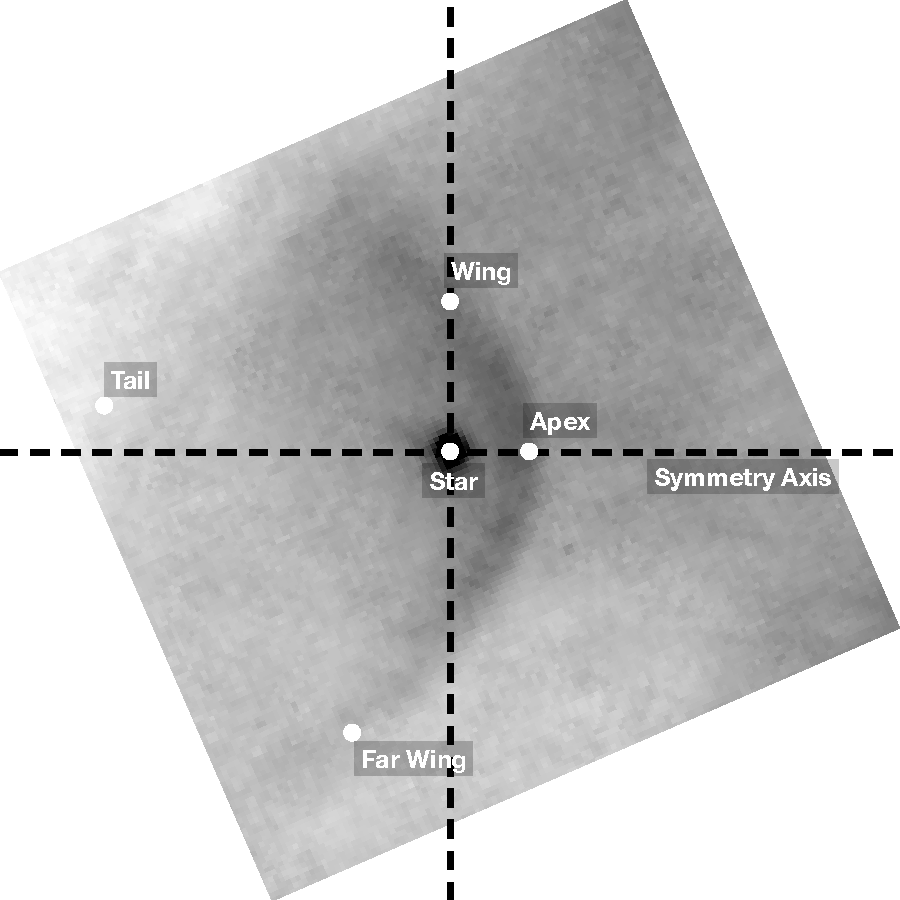
\includegraphics[width=0.9\linewidth]{figs/bow-terminology}
  \caption{Descriptive terminology for a stellar bow shock.  The apex
    is the closest approach of the bow to the star, while the wings
    are the parts of the bow that curve back past the star.}
  \label{fig:bow-terminology}
\end{figure}
A further class of astrophysical bow shock is driven by highly
collimated, supersonic jets of material, such as the Herbig Haro
objects \citep{Schwartz:1978b, Hartigan:1987a} that are powered by
jets from young stars or protostars.  Additional examples are seen in
planetary nebulae \citep{Phillips:2010a, Meaburn:2013a}, active
galaxies \citep{Wilson:1987a}, and in galaxy clusters
\citep{Markevitch:2002a}.  In the jet-driven case, the term ``working
surface'' is often applied to the entire structure comprising the two
shocks plus the shocked gas in between them, separated by a
\textit{contact discontinuity}.  The working surface may be due to the
interaction of the jet with a relatively quiescent medium, or may be an
``internal working surface'' within the jet that is due to
supersonic temporal variations in the flow velocity
\citep{Raga:1990a}.

In empirical studies the relationship between these theoretical
constructs and the observed emission structures is not always clear.
In such cases the term ``bow shock'' is often used in a more general
sense to refer to the entire arc of emission.  In this paper, we will
concentrate on \textit{stellar bow shocks}, in which the position of
the star can serve as a useful reference point for describing the bow
shape.  The empirical terminology that we will employ is illustrated
in Figure~\ref{fig:bow-terminology}.  The \textit{apex} is the point
of closest approach of the bow to the star, which lies on the
approximate symmetry axis, and the region around the apex is sometimes
referred to as the \textit{head} of the bow.  The \textit{wings} are
the swept-back sides of the bow, which lie in a direction from the
star that is orthogonal to the axis, with the \textit{far wings} being
the wing region farthest from the apex. Finally, the \textit{tail} is
the region near the axis but in the opposite direction from the apex.



Bow shocks from pulsars and neutron stars
\citep{Cordes:1993a, Brownsberger:2014a}. 

Terminology: head, wings, nose, apex, limb, etc. 




Radiative versus non-radiative shocks. 


\begin{figure}
  % 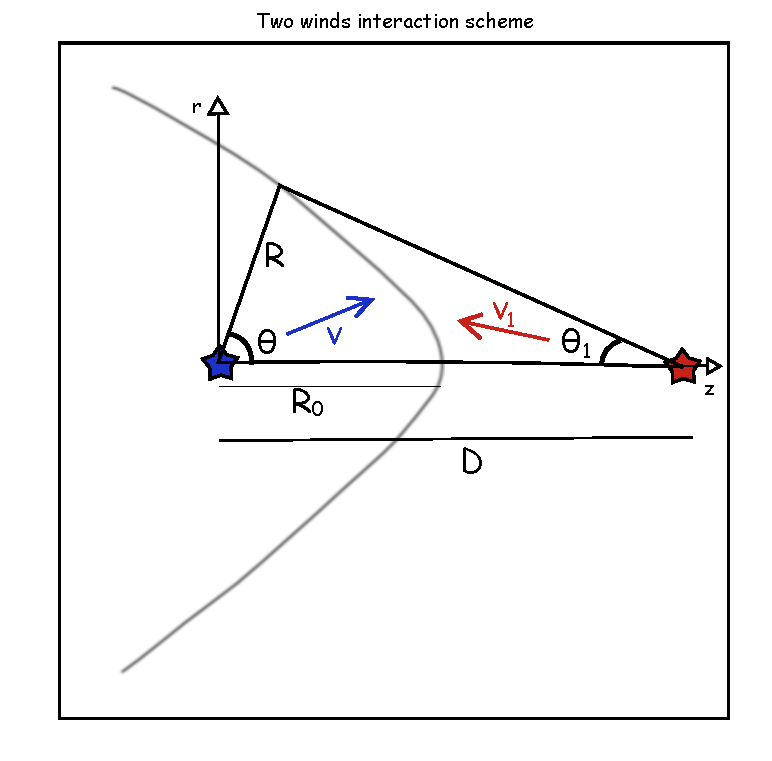
\includegraphics[width=\linewidth]{2winds-scheme}
  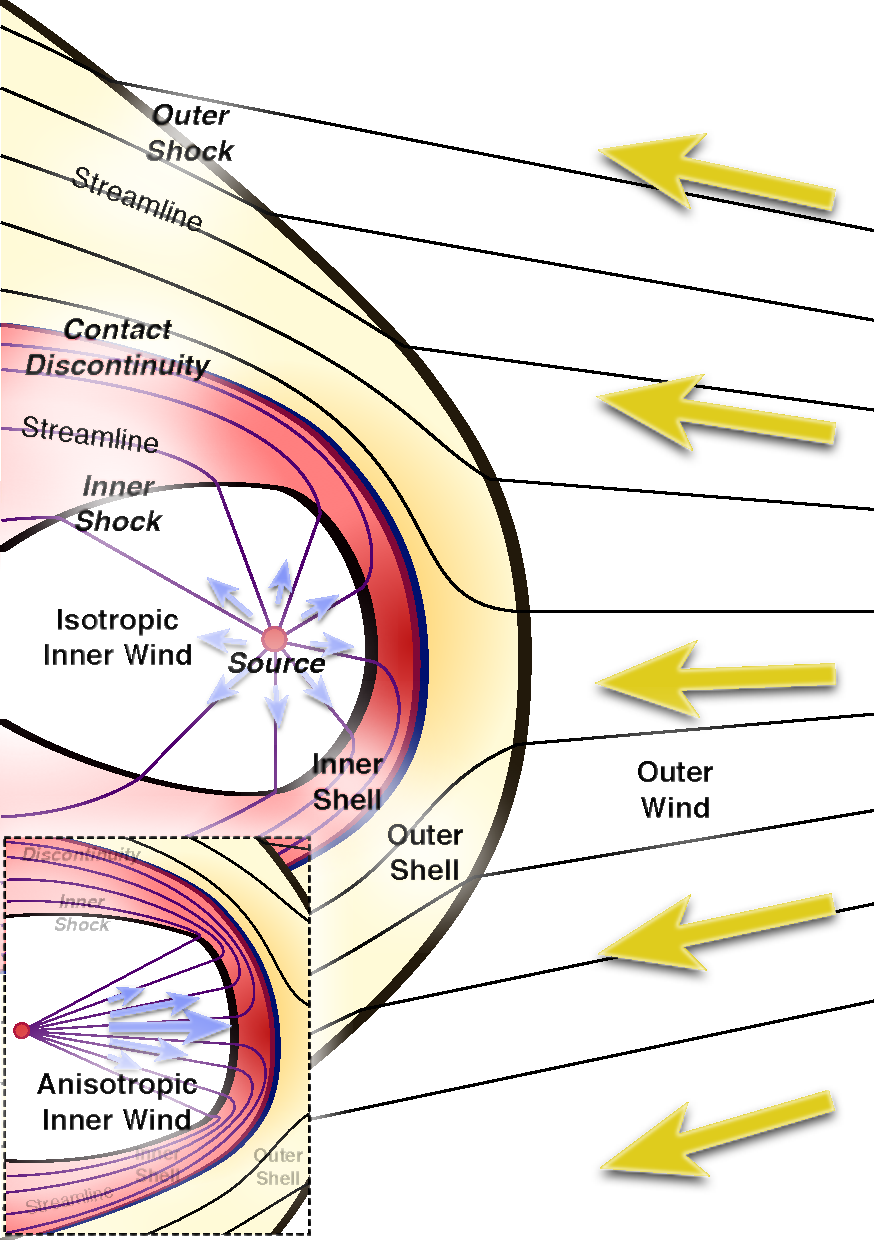
\includegraphics[width=\linewidth]{figs/generic-bowshock}
  \caption{Quasi-stationary bow shock structure formed by the
    interaction of two supersonic winds.  Lower-left inset box shows
    the case where the inner wind is anisotropic. The streamlines
    (thin lines) are drawn to be qualitatively realistic: they
    are straight in regions of hypersonic flow, but curved in subsonic
    regions, responding to pressure gradients in the shocked shells.}
\label{fig:2-winds}
\end{figure}
can't doesn;t 
\begin{figure}
  \centering
  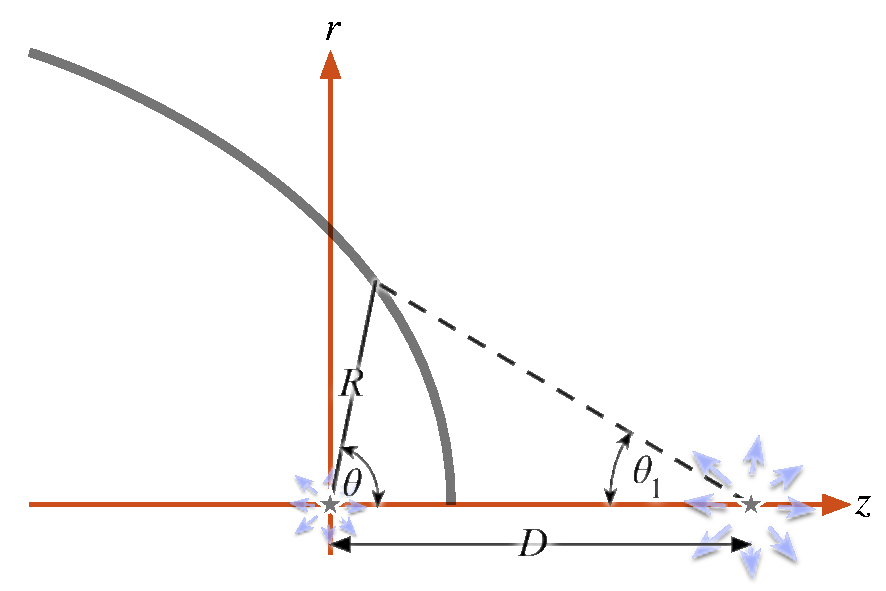
\includegraphics[width=\linewidth]{figs/bowshock-crw-variables}
  \caption[]{Schematic diagram of two-wind interaction problem,
    following \citet{Canto:1996}.}
  \label{fig:crw-schema}
\end{figure}

The general case of a two-wind interaction bow shock is illustrated in
Figure~\ref{fig:2-winds}.  If the winds are isotropic, then the bow
shock pattern wraps around the weaker of the two sources, in

The bow shocks we consider are originated by a source located at the
origin, emitting a wind with a mass loss rate of $\dot{M}_w$ and a
terminal (supersonic) velocity $v_w$. This wind interacts with another
wind originated by another source located at a distance $D$ from the
first one.  The mass loss rate of the second source is $\dot{M}_{w1}$
and the terminal velocity is $v_{w1}$. The momentum of the wind of the
second source is higher than the momentum of the first one, and the
resultant bow shock is stationary due to pressure balance.

\subsection{Characteristic Radii}
\begin{figure}
  \centering
  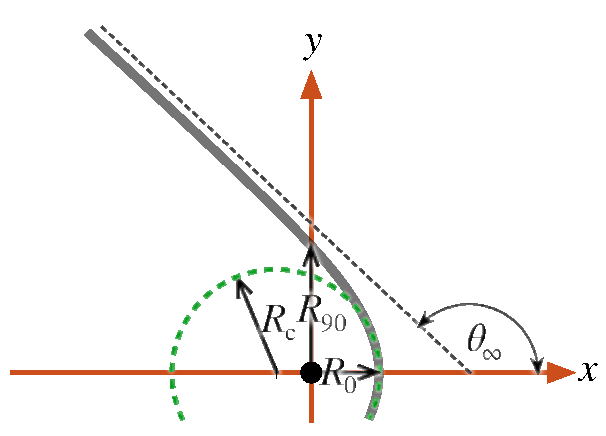
\includegraphics[width=\linewidth]{figs/characteristic-radii}
  \caption{Characteristic radii in the body frame.}
  \label{fig:characteristic-radii}
\end{figure}


In order to contrast different bow shock models, we derive a set of
measurable radii. Each model used should predict them and these
predictions can be compared with observations.
\begin{itemize}
\item Radius at axis of symmetry. Denoted as $R_0$.
\item Radius of Curvature at the axis of symmetry. Denoted as $R_c$
\item Radius at the perpendicular direction to the symmetry
  axis. Denoted as $R_{90}$
\item For open bow shocks, the asymptotic angle. Denoted as
  $\theta_\infty$
\end{itemize}



%% 
%% Restriction to cylindrical symmetry
%% 

For simplicity, the current paper is restricted to cylindrically
symmetric bow shock shapes. 

%%
%% Effects of instabilities
%%


%%% Local Variables:
%%% mode: latex
%%% TeX-master: "quadrics-bowshock"
%%% End:
